\section {IMU Cluster}
В настоящее время широкое распространение получили блоки инерциальных чувствительных элементов на базе MEMS-технологии.
Их основными преимуществами являются: низкая стоимость, малые массогабаритные характеристики и низкое энергопотребление.
Однако подобные приборы обладают низкой точностью: нестабильность нуля у гироскопов единицы-десятки градусов в час, а у акселерометров сотые-деястые доли милли-g.

Одним из путей повышения точности микромеханических бчэ является объединение их в массив (кластер). [ссылки на работы по кластеру].
Кластерные бчэ позволяют уменьшить шум в информационном сигнале в $\sqrt{N}$ раз, где $N$ - количество отдельных используемых бчэ. [ссылка]

\newpage

Для проверки и подтверждения характеристик кластерного бчэ в ходе данной работы была создана печатная плата (Рис. \ref{fig:cluster_pcb}).

\begin{figure}[h!]
	\centering
	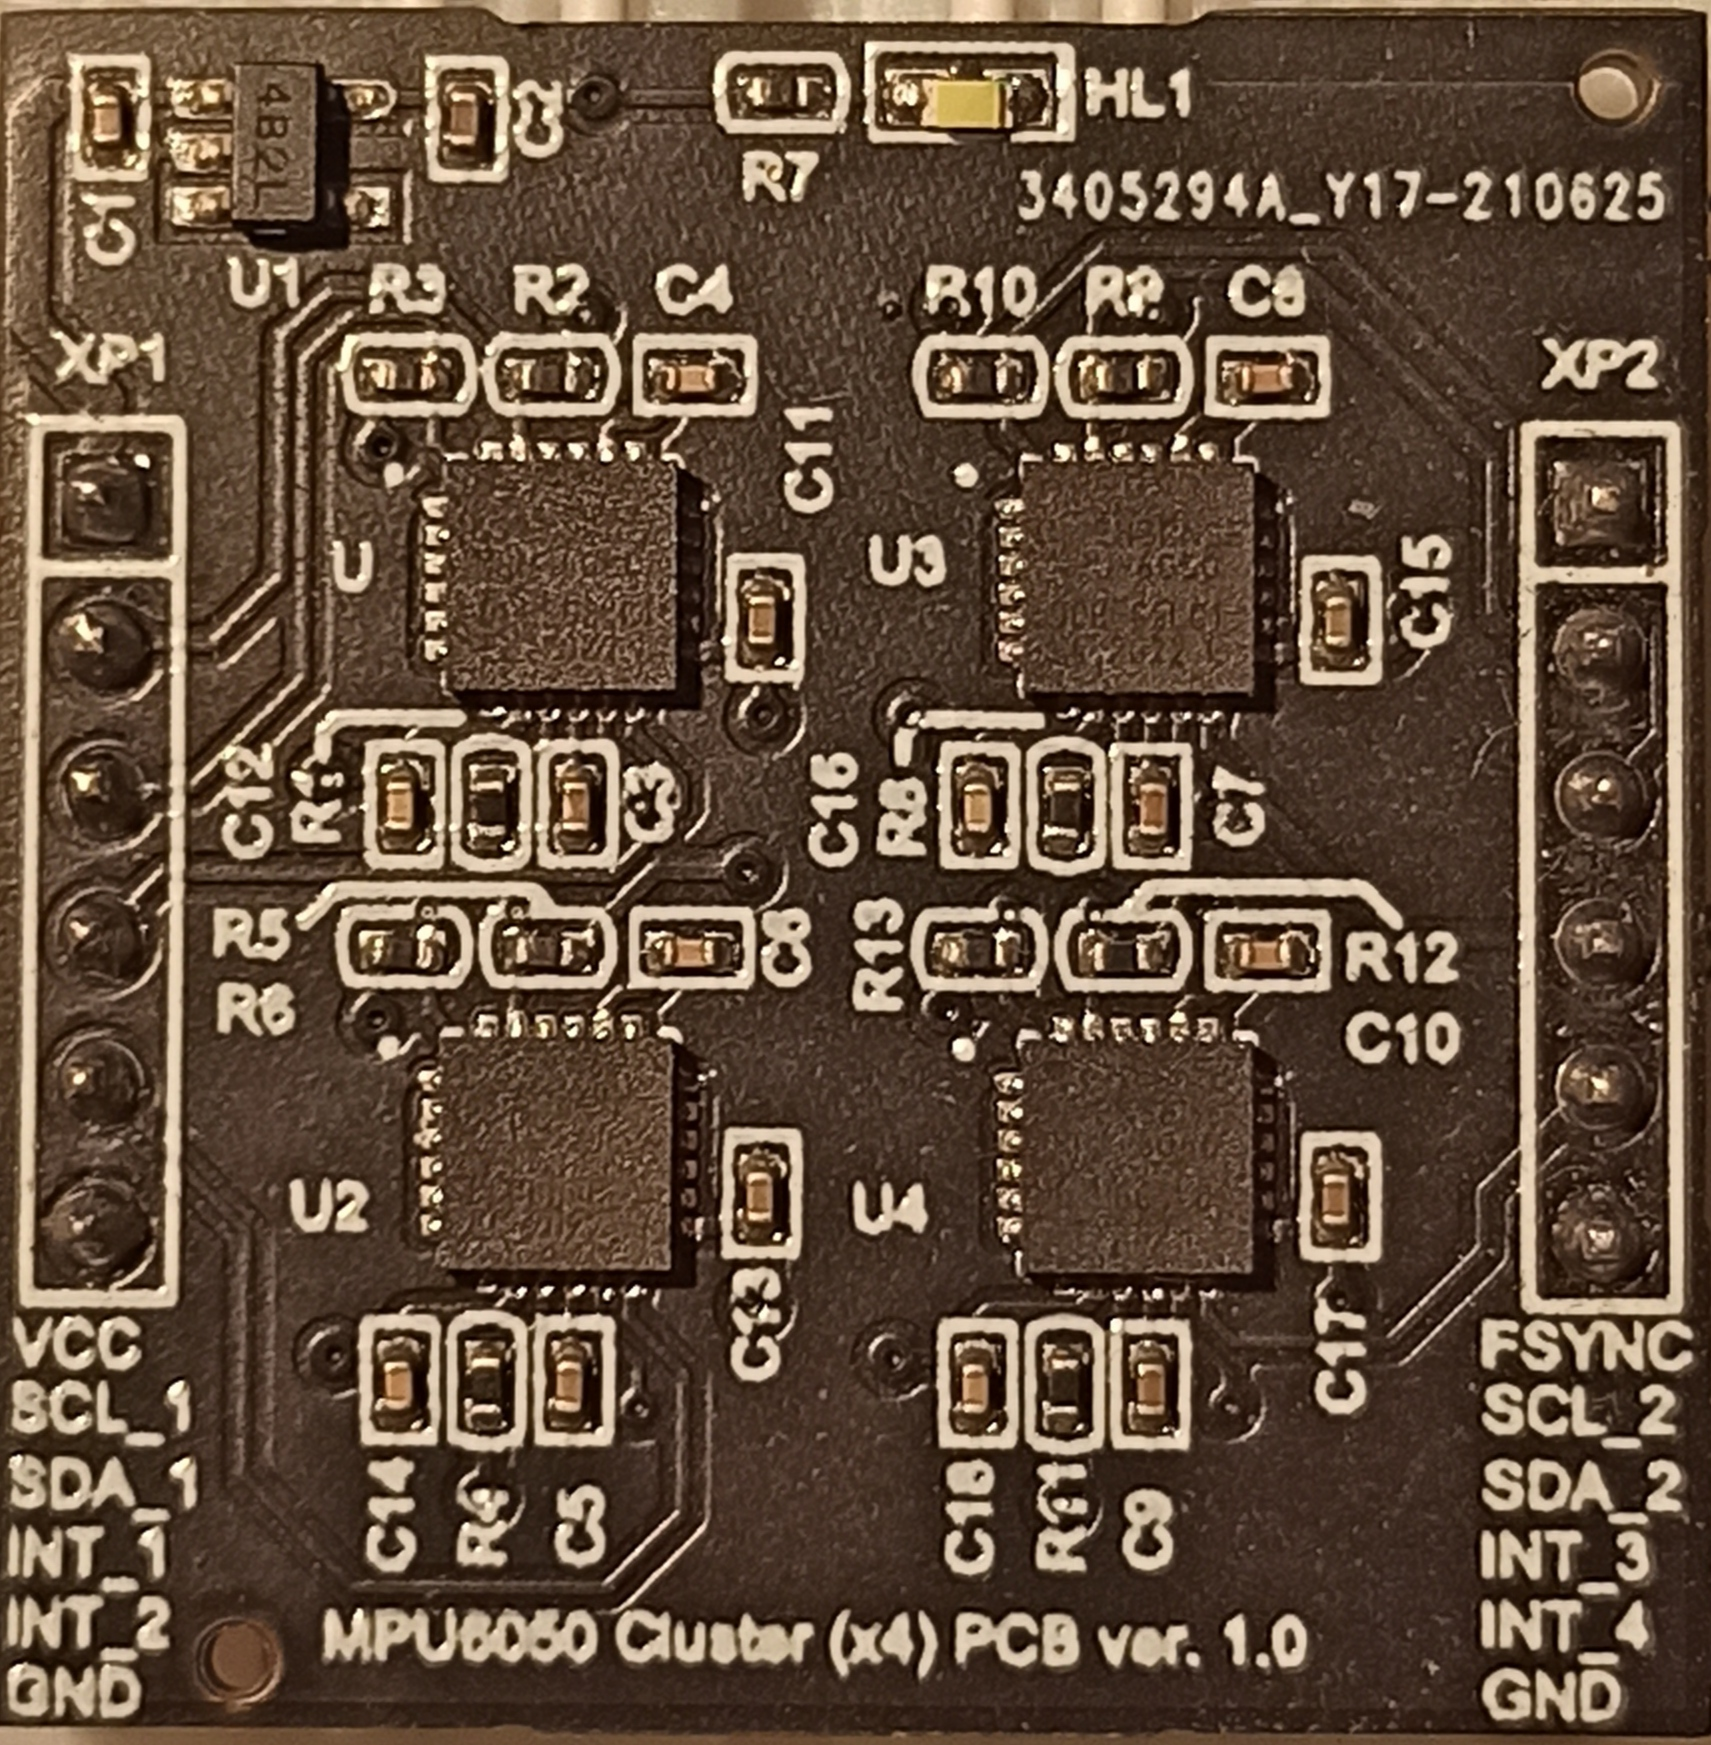
\includegraphics[width=0.4\linewidth]{cluster_pcb.jpg}
	\caption{Печатная плата с кластерным БЧЭ}
	\label{fig:cluster_pcb}
\end{figure}

В состав разработанного кластерного БЧЭ входят шестиосные датчики фирмы Invensense MPU6050 (трехосный акселерометр и трехосный датчик угловых скоростей).
Данные БЧЭ были выбраны вследствие их наибольшей распространнености и доступности.
Каждый из MPU6050 располагается на печатной плате в вершинах квадрата со стороной 10 мм.
Кроме того, они установлены так, чтобы соответствующие оси чувстительности каждого датчика были параллельны между собой.

Характеристики макетной платы с четырьмя MPU6050. Графики девиации Аллана. Сводная таблица погрешностей IMU.